\documentclass[german]{latteachCD}
\usepackage{mdframed}
\usepackage{amsmath}
\usepackage{amsfonts}
\usepackage{amssymb}
\usepackage{fdsymbol}
%\usepackage{wasysym}
%\usepackage{stmaryrd}
%\usepackage{fixltx2e}
%\usepackage{enumitem}
%\usepackage{extarrows}
%\newcommand{\abs}[1]{\lvert#1\rvert}

\usepackage{tikz}
\usetikzlibrary{arrows,automata,positioning,shapes,calc,decorations.pathmorphing,matrix}

\tikzstyle{automaton}=[->, >=stealth', initial text=, auto, node distance=20mm, bend angle=20, semithick, x=20mm, y=20mm]
\tikzset{
  every state/.style={
    inner sep=0pt,
    minimum size=8mm
  },
  small state/.style={
      state,
      minimum size=3mm
  },
  ellipse state/.style={
    draw,
    shape=ellipse,
    minimum width=20mm,
    minimum height=12.36mm,
    text width=14.5mm,
    inner sep=0mm,
    path picture={
      \draw (path picture bounding box.east) ellipse [x radius=9mm, y radius=9mm];
    }
  },
  accepting ellipse state/.style={
    ellipse state,
    path picture={
      \clip (path picture bounding box.east) ellipse [x radius=9.4mm, y radius=9.4mm];
      \draw[double] (path picture bounding box.east) ellipse [x radius=9mm, y radius=9mm];
      \draw[double] (path picture bounding box.center) ellipse [x radius=10mm, y radius=6.18mm];
    }
  }
}


\newcommand{\T}{\ensuremath\mathcal{M}}
\newcommand{\bin}{\ensuremath\mathit{bin}}
\newcommand{\poly}{\text{\normalfont poly}}

%%%%%%%%%%%%%%%%%%%%%%%%%%%%%%%%%%%%%%%%%%%%%%%%%%%%%%%%%%%%%%%%%%%%%%%%%%%%%%%%%%%%%%%%%%%%

\usepackage{xspace}

\author{~}
\term{Wintersemester 2017/18}
\title{\Large 10.\@ Übungsblatt}
\course{\LARGE Formale Systeme}

\usepackage{csquotes}
\usepackage{booktabs}
\usepackage{amsmath}
\usepackage{amsfonts}
\usepackage{amssymb}
\usepackage{mathtools}
\usepackage{wasysym}
\usepackage{stmaryrd}
\usepackage{enumitem}
\usepackage{tikz}
\usepackage{makecmds}

\renewcommand{\epsilon}{\varepsilon}
\renewcommand{\phi}{\varphi}
\renewcommand{\rho}{\varrho}
\renewcommand{\theta}{\vartheta}
\newcommand{\tuple}[1]{\langle{#1}\rangle} 

\newcommand{\size}[1]{\ensuremath{\lvert #1\rvert}}
\newcommand{\gdw}{\mathrel{\mathrm{gdw.}}}
\newcommand{\falls}{\mathrel{\mathrm{falls}}}

\provideenvironment{solution}{\textbf{Lösung}:}{}
\usepackage{comment}

\usepackage{etex,etoolbox}

\DeclareRobustCommand{\NN}{\ensuremath{\mathbb{N}}}

\newbool{Baader}
\newbool{Kroetzsch}
\booltrue{Kroetzsch}

\DeclareMathOperator{\Var}{Var}
\ifbool{Baader}{%
  \DeclareMathOperator{\Unt}{Unt}
  \DeclareMathOperator{\Res}{Res}
}{}
\ifbool{Kroetzsch}{%
  \DeclareMathOperator{\Unt}{Sub}
  \DeclareMathOperator{\Res}{Res}
  \usepackage{multicol}         % for resolution
}{}

\excludecomment{solution}

\begin{document}

\maketitle

%\begin{center}
%\begin{mdframed}
%  \renewcommand{\theexercise}{zur Selbstkontrolle
%  (diese werden in den Übungen nicht besprochen)}
%%  
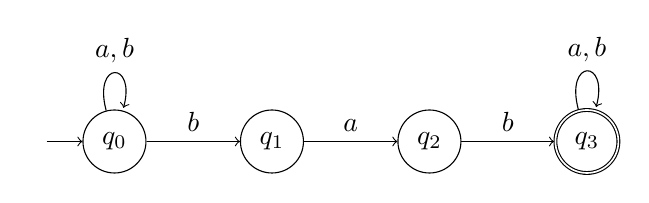
\begin{tikzpicture}[node distance=2cm, auto]
   \node[state,initial,initial text= ] (q0) {$q_0$};
   \node[state] (q1) [right of=q0] {$q_1$};
   \node[state] (q2) [right of=q1] {$q_2$};
   \node[state, accepting] (q3) [right of=q2] {$q_3$};

\path[->] (q0) edge [loop above] node {$a,b$} ()
               edge              node {$b$} (q1)
          (q1) edge              node {$a$} (q2)
          (q2) edge              node {$b$} (q3)
          (q3) edge [loop above] node {$a,b$} ()
;
\end{tikzpicture}

%%  {\bfseries Hinweis:} Die Aufgaben *) und **)
%%  dienen der Selbstkontrolle und werden in der
%%  Übung nicht besprochen.
%\end{mdframed}
%\end{center}

%\vspace*{0.5cm}
%{\bf{Anmerkung}}\\
%Mit der 9. \"Ubung ist in den verschiedenen \"Ubungsgruppen abzusichern, dass alle bisher aus Zeitgr\"unden noch nicht besprochenen Aufgaben der \"Ubungsbl\"atter 1 bis 8 abgearbeitet sind.

\setcounter{exercise}{0}

% diese aufgabe hat sich erledigt - wurde in vl komplett gezeigt:
%\input{pool/sprachen-turingmaschine-zweierpotenz}

% Zur Widerholung beim nächsten Mal...
%\input{pool/sprachen-turingmaschine-ai_bi_ci}

\begin{exercise}

Gegeben ist die nichtdeterministische $3$-Band Turingmaschine
 $$\T \ = \ (\{q_0,q_1,q_2\}, \{a,b\}, \{a,b,\Box\}, \delta,q_0,
\Box,\{q_2\})
$$
mit
$$\begin{array}{lcl}
  \delta(q_0, a,\Box,\Box) & = & \{ (q_0, \langle a,R\rangle, \langle  a,R
  \rangle ,\langle  \Box,N  \rangle ), \\
  &  &  (q_1, \langle a,R\rangle, \langle  a,N
  \rangle ,\langle  \Box,L  \rangle )   \} \\
  
  \delta(q_0, b,\Box,\Box) & = & \{ (q_0, \langle b,R\rangle, \langle  \Box,N
  \rangle ,\langle  b,R  \rangle ), \\
  &  &  (q_1, \langle b,R\rangle, \langle  \Box,L
  \rangle ,\langle  b,N  \rangle )    \} \\

  \delta(q_1, a,a,b) & = & \{ (q_1, \langle a,R\rangle, \langle  \Box,L
  \rangle ,\langle  b,N  \rangle )    \} \\

  \delta(q_1, a,a,\Box) & = & \{ (q_1, \langle a,R\rangle, \langle  \Box,L
  \rangle ,\langle  \Box,N  \rangle )    \} \\

  \delta(q_1, b,a,b) & = & \{ (q_1, \langle b,R\rangle, \langle  a,N
  \rangle ,\langle  \Box,L  \rangle )    \} \\

  \delta(q_1, b,\Box,b) & = & \{ (q_1, \langle b,R\rangle, \langle  \Box,N
  \rangle ,\langle  \Box,L  \rangle )    \} \\

  \delta(q_1, \Box,\Box,\Box) & = & \{ (q_2, \langle \Box,N\rangle, \langle  \Box,N
  \rangle ,\langle  \Box,N  \rangle )    \} \\

\end{array}
$$

Welche Sprache akzeptiert $\T$ ? 
Hinweis: Sie können die Arbeitsweise von
$\T$ gerne mithilfe einer graphischen 
Repräsentation der Übergangsrelation~$\delta$ 
nachvollziehen.

\end{exercise}

\begin{exercise}
	
Geben Sie pr\"azise eine deterministische Turingmaschine $\T$ zur Erkennung der Sprache 
$L \ = \  \bigl\{ a^nb^mc^k: n,m,k \geq 1, n=2m  \ \text{oder} \ m = k\}$ an.
Sie k\"onnen wahlweise eine Ein- oder Mehrband-DTM verwenden.

\begin{itemize}
\item [(a)]

Begr\"unden Sie, warum ${\mathcal L}(\T) = L$. 

\item [(b)]
Geben Sie die Berechnungen f\"ur $w_1 = abcc$ und $w_2 = aabc$ an.
\end{itemize}
\end{exercise}



\begin{exercise}
Wie in der Vorlesung dargelegt wurde, werden Turingmaschinen als allgemeines Rechenmodell verstanden (18.\,Vorlesung, Folie 19).\\[0.2cm]
Geben Sie Turingmaschinen an, die folgende Funktionen 
berechnen. Dabei wird eine Eingabe $n\in \mathbb N$ als $\emptyset^n$ mit $\emptyset\in \Sigma$ dargestellt. Es kann vorausgesetzt werden, dass die Eingabe wohlgeformt auf dem Band vorliegt. Am Ende der Berechnung h\"alt die Turingmaschine in einem Finalzustand und das Band enth\"alt nur das Berechnungsergebnis. 
\begin{enumerate}
\item[a)] Die Turingmaschine $\mathcal M_{0}$ berechnet die
  Funktion $f:\mathbb N\rightarrow \mathbb N,\,n\mapsto 0$, d.\,h. das Eingabewort auf dem
  Band wird gelöscht.
\item[b)] Die Turingmaschine $\mathcal M_{succ}$ berechnet die
  Funktion $f:\mathbb N\rightarrow \mathbb N,\,n\mapsto n+1$.
\item[c)] Für $i,n\in \mathbb N$ berechnet die Turingmaschine $\mathcal M_{n}^i$
  die Funktion $f^i_n:\mathbb N^n\rightarrow \mathbb
  N$ mit $(x_1,\ldots,x_n)\mapsto x_i$. Es wird empfohlen, zunächst die
  Turingmaschine $\mathcal M_{4}^2$ anzugeben und diese dann zu
  $\mathcal M_{n}^i$ zu verallgemeinern.\\[1ex]
  \textit{Hinweis}: $(3,2,4,0)$ in der Eingabe wird dargestellt als \mbox{$(\emptyset\emptyset\emptyset,\emptyset\emptyset,\emptyset\emptyset\emptyset\emptyset,)\textvisiblespace$ }. 
\end{enumerate} 
\end{exercise}



%%%%%%%%%%%%%%%%%%%%%%%%%%%

% zu komplex für den moment
%\input{pool/baier/14b}

%%%%%%%%%%%%%%%%%%%%%%%%%%%

\end{document}
